
\begin{frame}
 \frametitle{Demo 8-1 $\vert$ \bfseries Transversal isotropy}
 \framesubtitle{\bfseries tension test of glass-fiber reinforced plastic}
 \only<2>{\framesubtitle{\bfseries compliance matrix for \(\v a = \v e_1\)}}
 \only<3>{\framesubtitle{\bfseries elasticity matrix for \(\v a = \v e_1\)}}
  \begin{overlayarea}{0.9\textwidth}{0.9\textheight}
 \vspace*{-5ex}
 \begin{center}
 \hspace*{-1em}
 \begin{tikzpicture}[scale=3]
 \onslide<1>{
 \fill[gray!10] (0, 1) rectangle (1, 0);
 \begin{scope}
  \clip (0, 1) rectangle (1, 0);
 \foreach \y in {-1.0, -0.9, ..., 1.0}
  \draw[gray!30,ultra thick,rotate=45] (-1, \y) -- +(3, 0);
 \end{scope} 
 \draw (0, 1) rectangle (1, 0) node[above left, black]{$\mathcal{B}$};

  \draw[thin,gray] (0, 1) -- +(0, 0.2);
  \draw[thin,gray] (1, 1) -- +(0, 0.2);
  \draw[<->,thin,gray] (0, 1.15) -- node[fill=white]{$\ell$} +(1, 0);
  \draw[thin,gray] (1, 0) -- +(0.6, 0);
  \draw[thin,gray] (1, 1) -- +(0.6, -0);
  \draw[<->,gray] (1.55, 0) -- node[fill=white,sloped]{$\ell$} +(0, 1);

  \draw[thick,-latex] (0, 0) -- +(0.5, 0) node[below]{$\v e_1$};
  \draw[thick,-latex] (0, 0) -- +(0, 0.5) node[right]{$\v e_2$};
  \draw[thick,-latex] (0, 0) -- (0.386, 0.386) node[right]{$\v a$};
  \draw (0.25,0) arc (0:45:0.25cm) node[below=3pt,xshift=-2pt]{$\alpha$};

  \foreach \x in {0.0,0.1666,0.333,...,1.0}
  \draw[thick,-latex] (1, 0.05+0.9/1.0*\x) -- +(0.2, 0);
  \node at (1.2, 0.8) [right,xshift=0.0cm]{$\v u^p$};

  \fill[pattern=north west lines, pattern color=black] (-0.1, -0.0) rectangle +(-0.1, 1.0);
  \draw[thick] (-0.1, -0.0) -- +(0, 1.0);
  \draw[yshift=0.1cm] (0, 0) -- +(-0.07, 0.06) -- +(-0.07, -0.06) -- (0,0) +(-0.07, -0.1) -- +(-0.07, 0.1);
  \draw[yshift=0.9cm] (0, 0) -- +(-0.07, 0.06) -- +(-0.07, -0.06) -- (0,0) +(-0.07, -0.1) -- +(-0.07, 0.1);

   \fill[pattern=north west lines, pattern color=black] (-0.1, -0.07) rectangle +(0.2, -0.05);
   \draw[thick] (-0.1, -0.07) -- +(0.2, 0);
  \draw[xshift=0.00cm,rotate=90] (0, 0) -- +(-0.07, 0.06) -- +(-0.07, -0.06) -- (0,0) +(-0.07, -0.1) -- +(-0.07, 0.1);
%   \draw[xshift=0.95cm,rotate=90] (0, 0) -- +(-0.07, 0.06) -- +(-0.07, -0.06) -- (0,0) +(-0.07, -0.1) -- +(-0.07, 0.1);

%   \fill[pattern=north west lines, pattern color=black] (3, -0.25) rectangle +(0.25, 1.5);
%   \draw[thick] (3, -0.25) -- +(0, 1.5);
  }
  \onslide<2>{
  \node at (-0.2, 0.6) [right]{\parbox{8cm}{
 \[
 \begin{bmatrix}
  \varepsilon_{11} \\[1ex] \varepsilon_{22} \\[1ex] \varepsilon_{33} \\[1ex]
  2\varepsilon_{23} \\[1ex] 2\varepsilon_{13} \\[1ex] 2\varepsilon_{12}
 \end{bmatrix}
 \!=\!
 \begin{bmatrix}
 \frac{1}{E_\parallel} & -\frac{\nu_{\parallel \perp}}{E_\parallel} & -\frac{\nu_{\parallel \perp}}{E_\parallel} & 0 & 0 & 0\\[1ex]
 -\frac{\nu_{\parallel \perp}}{E_\parallel} & \frac{1}{E_\perp} & -\frac{\nu_{\perp \perp}}{E_\perp} & 0 & 0 & 0\\[1ex]
 -\frac{\nu_{\parallel \perp}}{E_\parallel} & -\frac{\nu_{\perp \perp}}{E_\perp} & \frac{1}{E_\perp} & 0 & 0 & 0\\[1ex]
 0 & 0 & 0 & \frac{1}{\mu_{\perp \perp}} & 0 & 0 \\[1ex]
 0 & 0 & 0 & 0 & \frac{1}{\mu_{\parallel \perp}} & 0 \\[1ex]
 0 & 0 & 0 & 0 & 0 & \frac{1}{\mu_{\parallel \perp}}
\end{bmatrix} 
 \!
 \begin{bmatrix}
  \sigma_{11} \\[1ex] \sigma_{22} \\[1ex] \sigma_{33} \\[1ex]
  \sigma_{23} \\[1ex] \sigma_{13} \\[1ex] \sigma_{12}
 \end{bmatrix}
\]
   }};
   
   \node at (2.0, -0.2) [right,font=\footnotesize]{\parbox{4cm}{
    \[
     \text{with} \quad \nu_{\perp \perp} = \frac{E_\perp}{2 \mu_{\perp \perp}} - 1 = 0.3
    \]
   }};
   
  }
 \onslide<3>{
  \node at (-0.2, 0.7) [right,font=\footnotesize]{\parbox{8cm}{
 \[
 \begin{bmatrix}
  \sigma_{11} \\[1ex] \sigma_{22} \\[1ex] \sigma_{33} \\[1ex]
  \sigma_{23} \\[1ex] \sigma_{13} \\[1ex] \sigma_{12}
 \end{bmatrix} 
 \!=\!
 \begin{bmatrix}
 \frac{E_\parallel [1-\nu_{\!\perp \!\perp}^2]}{D} \! & \! \frac{E_{\!\perp} \nu_{\parallel \!\perp} [1+\nu_{\!\perp \!\perp}]}{D} \! & \! \frac{E_{\!\perp} \nu_{\parallel \!\perp} [1+\nu_{\!\perp \!\perp}]}{D} \! & \! 0 \! & \! 0 \! & \! 0\\[1ex]
 \frac{E_{\!\perp} \nu_{\parallel \!\perp} [1+\nu_{\!\perp \!\perp}]}{D} \! & \! \frac{E_{\!\perp} [1-\nu_{\parallel \!\perp}\nu_{\!\perp \parallel}]}{D} \! & \! \frac{E_{\!\perp} [\nu_{\!\perp \!\perp}+\nu_{\parallel \!\perp}\nu_{\!\perp \parallel}]}{D} \! & \! 0 \! & \! 0 \! & \! 0\\[1ex]
 \frac{E_{\!\perp} \nu_{\parallel \!\perp} [1+\nu_{\!\perp \!\perp}]}{D} \! & \! \frac{E_{\!\perp} [\nu_{\!\perp \!\perp}+\nu_{\parallel \!\perp}\nu_{\!\perp \parallel}]}{D} \! & \! \frac{E_{\!\perp} [1-\nu_{\parallel \!\perp}\nu_{\!\perp \parallel}]}{D} \! & \! 0 \! & \! 0 \! & \! 0\\[1ex]
 0 \! & \! 0 \! & \! 0 \! & \! \mu_{\!\perp \!\perp} \! & \! 0 \! & \! 0 \\[1ex]
 0 \! & \! 0 \! & \! 0 \! & \! 0 \! & \! \mu_{\parallel \!\perp} \! & \! 0 \\[1ex]
 0 \! & \! 0 \! & \! 0 \! & \! 0 \! & \! 0 \! & \! \mu_{\parallel \!\perp}
\end{bmatrix}
 \!
\begin{bmatrix}
  \varepsilon_{11} \\[1ex] \varepsilon_{22} \\[1ex] \varepsilon_{33} \\[1ex]
  2\varepsilon_{23} \\[1ex] 2\varepsilon_{13} \\[1ex] 2\varepsilon_{12}
 \end{bmatrix}
\]
   }};
   
 \node at (-0.2, -0.1) [right,font=\footnotesize]{\parbox{8cm}{
 \[
 \text{with }
  D = [1+\nu_{\!\perp \!\perp}] [1 - \nu_{\!\perp \!\perp} - 2 \nu_{\parallel \!\perp} \nu_{\!\perp \parallel}] , \quad 
  \nu_{\!\perp \!\perp} = \frac{E_{\!\perp}}{2 \mu_{\!\perp \!\perp}} - 1 = 0.3, \quad
  \nu_{\!\perp \parallel} = \frac{E_{\!\perp}}{E_{\parallel}} \nu_{\parallel \!\perp} \approx 0.85
 \]
   }};   
  }
  
% 
%  \onslide<4>{
%   \node at (-0.2, 0.7) [right,font=\footnotesize]{\parbox{8cm}{
%  \[
%  \begin{bmatrix}
%   \sigma_{11} \\[1ex] \sigma_{22} \\[1ex] \sigma_{33} \\[1ex]
%   \sigma_{23} \\[1ex] \sigma_{13} \\[1ex] \sigma_{12}
%  \end{bmatrix} 
%  \!=\!
%  \begin{bmatrix}
%  E_{1111} \! & \! 2 \nu_{\parallel \!\perp} [\lambda+\mu_{\!\perp\!\perp}] \! & \! 2 \nu_{\parallel \!\perp} [\lambda+\mu_{\!\perp\!\perp}] \! & \! 0 \! & \! 0 \! & \! 0\\[1ex]
%  2 \nu_{\parallel \!\perp} [\lambda+\mu_{\!\perp\!\perp}] \! & \! \lambda+2\mu_{\!\perp\!\perp} \! & \! \lambda \! & \! 0 \! & \! 0 \! & \! 0\\[1ex]
%  2 \nu_{\parallel \!\perp} [\lambda+\mu_{\!\perp\!\perp}] \! & \! \lambda \! & \! \lambda+2\mu_{\!\perp\!\perp} \! & \! 0 \! & \! 0 \! & \! 0\\[1ex]
%  0 \! & \! 0 \! & \! 0 \! & \! \mu_{\!\perp \!\perp} \! & \! 0 \! & \! 0 \\[1ex]
%  0 \! & \! 0 \! & \! 0 \! & \! 0 \! & \! \mu_{\parallel \!\perp} \! & \! 0 \\[1ex]
%  0 \! & \! 0 \! & \! 0 \! & \! 0 \! & \! 0 \! & \! \mu_{\parallel \!\perp}
% \end{bmatrix}
%  \!
% \begin{bmatrix}
%   \varepsilon_{11} \\[1ex] \varepsilon_{22} \\[1ex] \varepsilon_{33} \\[1ex]
%   2\varepsilon_{23} \\[1ex] 2\varepsilon_{13} \\[1ex] 2\varepsilon_{12}
%  \end{bmatrix}
% \]
%    }};
%    
%  \node at (-0.2, -0.1) [right,font=\footnotesize]{\parbox{8cm}{
%  \[
%  \text{with }
%   E_{1111} = \frac{1 - \nu_{\!\perp \!\perp}}{1 - \nu_{\!\perp \!\perp} - 2 \nu_{\parallel \!\perp} \nu_{\!\perp \!\parallel}} E_{\parallel}, \quad
%   \lambda = \frac{\nu_{\parallel \!\perp} \nu_{\perp \!\parallel} + \nu_{\!\perp \!\perp}}{[1 - \nu_{\!\perp \!\perp} - 2 \nu_{\parallel \!\perp} \nu_{\!\perp \!\parallel}][1+ \nu_{\!\perp \!\perp}]} E_{\!\perp}
%  \]
%    }};   
%   }
  
  \onslide<1-3>{
  \node at (-0.2, -0.9) [right]{\parbox{4cm}{
   \begin{align*}
    E_{\parallel} &= 44 \, \mathrm{GPa} && \text{\scriptsize elast.\ mod.\ in fiber direction} \\
    E_{\perp} &= 13 \, \mathrm{GPa} && \text{\scriptsize elast.\ mod.\ in isotropic\ plane} \\ 
    \mu_{\parallel \perp} &= 5.6 \, \mathrm{GPa} && \text{\scriptsize shear mod.\ in planes parallel to fiber} \\
    \mu_{\perp \perp} &= 5.0 \, \mathrm{GPa} && \text{\scriptsize shear mod.\ in isotropic plane} \\
   \nu_{\parallel \perp} &= 0.25 && \text{\scriptsize Poisson's ratio for tension in fibre direction} \\
%    \nu_{\parallel} &= 0.3 && \text{\scriptsize elast.\ mod.\ in fibre direction}\\
   \end{align*}
   }};}
   \onslide<1>{
   \node at (2.3, -0.7) [right]{\parbox{4cm}{
   \begin{align*}
    [u^p_i] &= \begin{bmatrix} 0.02 \ell \\ 0 \\ 0 \end{bmatrix} \\[1ex]  \ell &= 1\,\mathrm{m}
   \end{align*}
   }};}
   
  \end{tikzpicture}
  \end{center}

 \end{overlayarea}
\end{frame}



\begin{frame}
 \frametitle{Demo 8-1 $\vert$ \bfseries Transversal isotropy}
 \framesubtitle{\bfseries tension test of glass-fiber reinforced plastic}
  \vspace*{-2ex}
  \hspace*{-2em}
  \begin{tikzpicture}
  \node at(0,0) {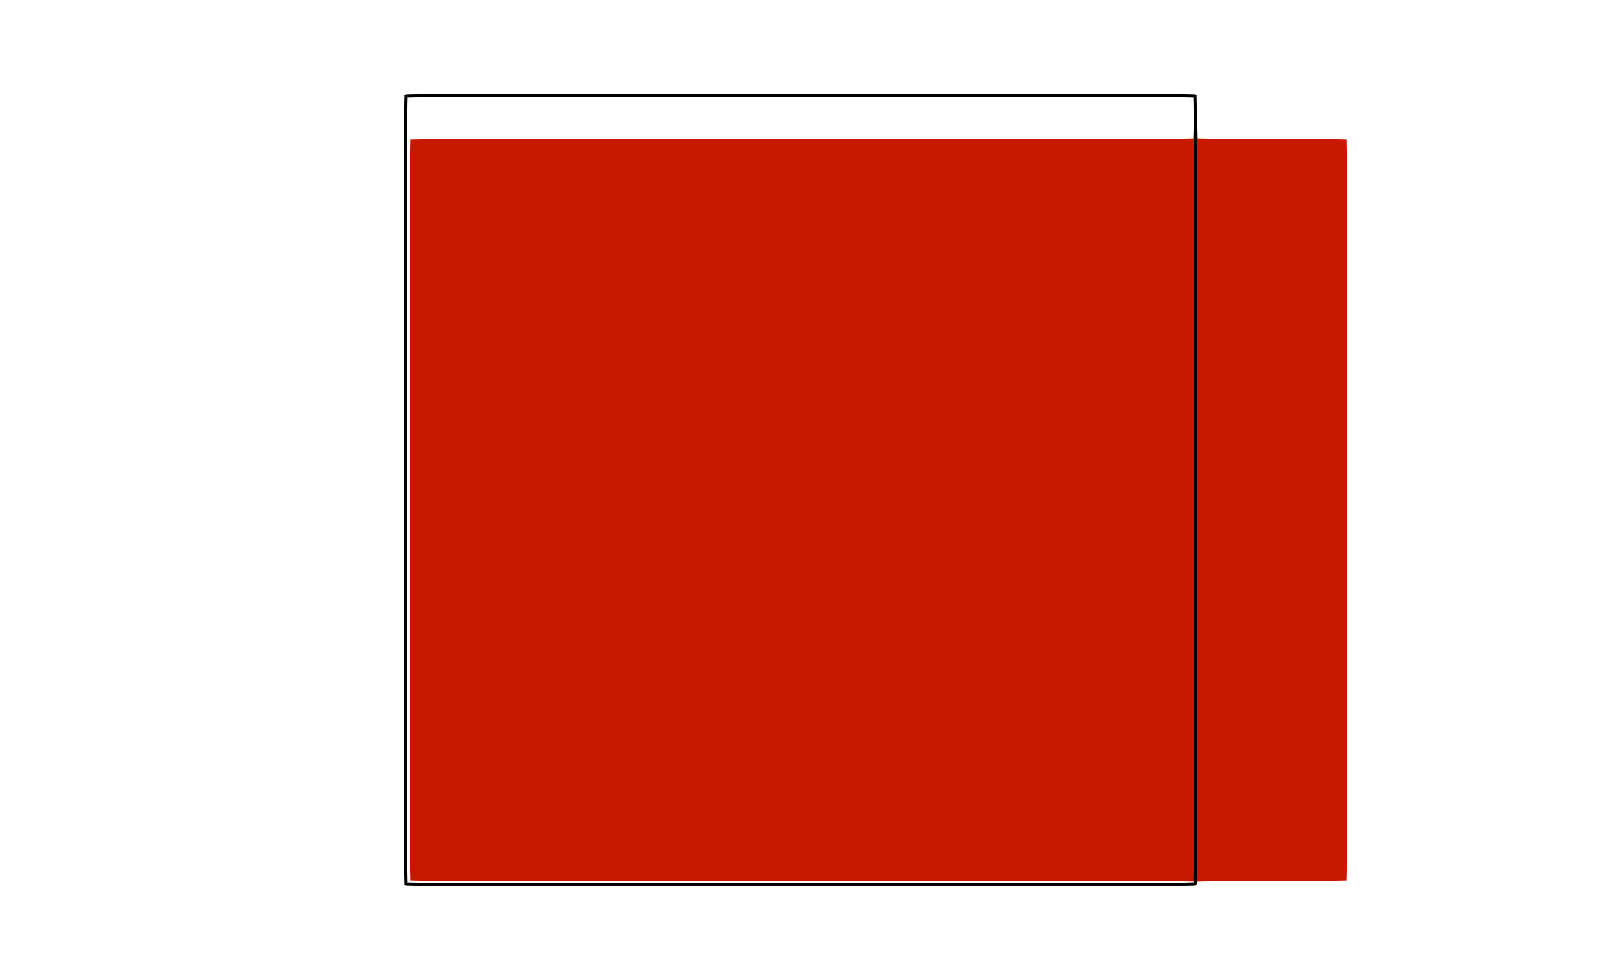
\includegraphics[width=5.8cm]{../09-anisotropy/tension2_0.png}};
  \node at(6,0) {
\includegraphics[width=5.8cm]{../09-anisotropy/tension2_90.png}};
  \node at(3,-3.5) {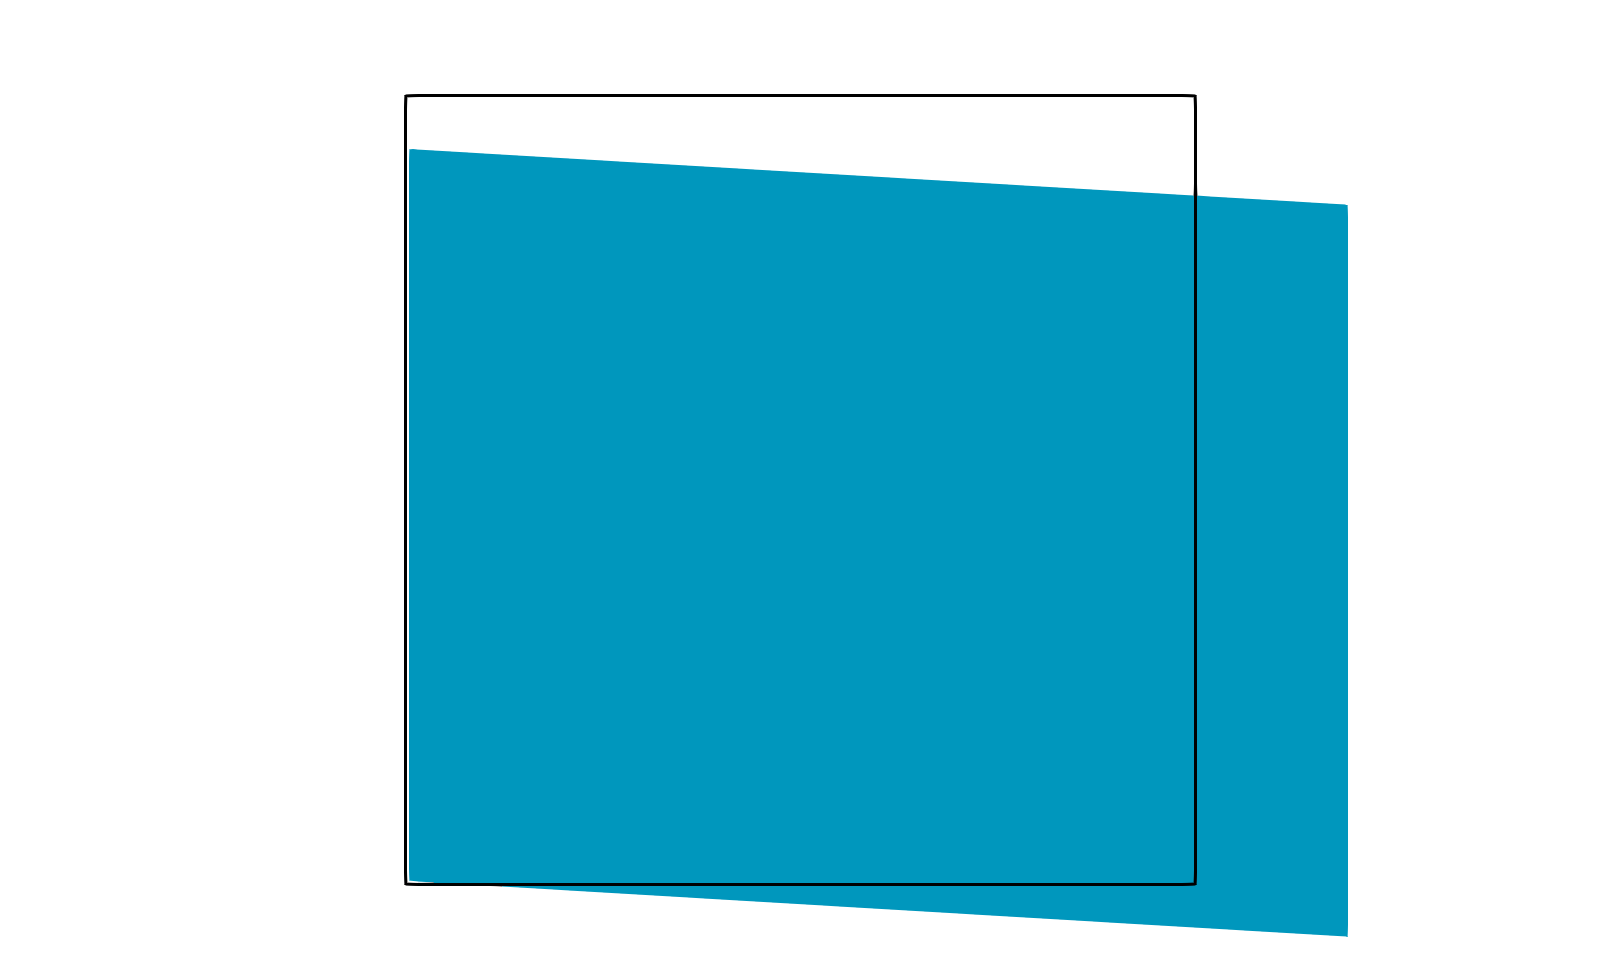
\includegraphics[width=5.8cm]{../09-anisotropy/tension2_45.png}};
%   \node at(6,-4) {
\includegraphics[width=6cm]{../08-isotropy/tension_-05.png}};
  
  \node at(-2.5, 0.5) {\(\alpha = 0^\circ\)};
  \node at(-2.5, -0.5) [font=\scriptsize]{\parbox{2cm}{
   \begin{align*}
    \sigma_{11} &= 680 \, \mathrm{MPa} \\
%     \varepsilon_{22} &= -0.005 
   \end{align*}}};
  \node at(3.5, 0.5) {\(\alpha = 90^\circ\)};
  \node at(3.5, -0.5) [font=\scriptsize]{\parbox{2cm}{
   \begin{align*} 
    \sigma_{11} &= 270 \, \mathrm{MPa} \\ 
%     \varepsilon_{22} &= -0.0019
   \end{align*}}};
  \node at(0.5, -3) {\(\alpha = 45^\circ\)};
  \node at(0.5, -4) [font=\scriptsize]{\parbox{2cm}{
   \begin{align*}
    \sigma_{11} &= 300 \, \mathrm{MPa} \\
%     \varepsilon_{12} &= -0.0071
   \end{align*}}};
   
%   \node at(3.5, -4) {\parbox{2cm}{\begin{align*} \nu &= -0.5 \end{align*}}};
%   \node at(3.5, -4.5) [font=\scriptsize]{(auxetic)};
  \begin{scope}[xshift=5.3cm,yshift=-2.5cm,scale=0.8]
   \begin{axis}[stressbar,point meta min=200,point meta max=700,title={$\sigma_{11}$ in $\mathrm{MPa}$}]
   \addplot [draw=none] coordinates {(0,0)}; \end{axis}
  \end{scope}   

  \node at (1, -6) [right,font=\footnotesize]{$\v u$ scaled with a factor of $10$};
 \end{tikzpicture}
\end{frame}

